% LaTeX source for ``การเรียนรู้ของเครื่องสำหรับเคมีควอนตัม (Machine Learning for Quantum Chemistry)''
% Copyright (c) 2022 รังสิมันต์ เกษแก้ว (Rangsiman Ketkaew).

% License: Creative Commons Attribution-NonCommercial-NoDerivatives 4.0 International (CC BY-NC-ND 4.0)
% https://creativecommons.org/licenses/by-nc-nd/4.0/

\chapter{การเลือกและปรับแต่งโมเดล}
\label{ch:reg_sel_model}

การทำให้โมเดลมีความสม่ำเสมอ (Regularization) เพื่อเพิ่มความถูกต้องและการเลือกโมเดล (Model Selection) เป็นสิ่งที่จำเป็นมากในขั้นตอน%
ของการฝึกสอนโมเดล

%--------------------------
\section{Cross Validation}
\label{sec:cross_val}
\idxen{Cross Validation}
%--------------------------

วิธีการตรวจสอบโมเดลวิธีแรกนี้เป็นวิธีที่ได้รับความนิยมเป็นอย่างมากเพราะว่าสามารถทำได้ง่ายและให้ผลลัพธ์ที่น่าเชื่อถือ นั่นก็คือ 
\enquote{K-Fold Cross Validation} หรือเรียกสั้น ๆ ว่า Cross Validation วิธีนี้เริ่มด้วยการแบ่งข้อมูล $k$ ให้มีขนาดของแต่ละส่วนเท่า ๆ กัน 
หลังจากนั้นทำเก็บข้อมูลหนึ่งส่วนไว้ใช้สำหรับเป็นตัวทดสอบโมเดลนั่นก็คือการทำ Validation แล้วทําวนไปเช่นนี้จนครบจํานวนที่แบ่งไว้ เช่น 
การทดสอบด้วยวิธี 5-fold Cross Validation ในรอบแรกเราจะทำการเทรนโมเดลด้วยชุดข้อมูลที่เกิดจากการวมส่วนที่ 2, 3, 4, และ 5 
และทำการทดสอบด้วยข้อมูลส่วนที่ 1 และในรอบที่สองเราจะเปลี่ยนมาเทรนโมเดลด้วยข้อมูลของส่วนที่ 1, 3, 4, และ 5 แล้วนำโมเดลมาทดสอบ%
ด้วยข้อมูลส่วนที่ 2

%--------------------------
\section{การคัดเลือกลักษณะเฉพาะ}
\label{sec:select_feat}
\idxen{Feature Selection}
%--------------------------

\begin{algorithm}[ht]
    \caption{อัลกอริทึม Forward Search สำหรับการทำ Feature Selection}
    \label{alg:forward_search}
    \begin{algorithmic}
    \State Initialize $\mathcal{F} = \emptyset$.
    \Repeat
        \For{$i=1,\ldots,d$}
            \If{$i \not\in \mathcal{F}$}
                \State $\mathcal{F}_i = \mathcal{F} \cup \{i\}$
                \State Use some version of cross validation to evaluate features $\mathcal{F}_i$.
                \State (i.e., train your learning algorithm using only the features in $\mathcal{F}_i$, and 
                estimate its generalization error.)
            \EndIf
        \EndFor
        \State Set $\mathcal{F}$ to be the best feature subset found in the previous step. % DIFF.
    \Until{convergence}
    \State Select and output the best feature subset that was evaluated during the entire search procedure.
    \end{algorithmic}
\end{algorithm}

การคัดเลือกลักษณะเฉพาะ (Feature Selection) เป็นการหา Feature ที่เหมาะสมที่สุดสำหรับการใช้อธิบายข้อมูลของโมเลกุล โดยเราจะทำการ%
เรียงลำดับความสำคัญของ Feature แล้วทำการคัดเลือกเฉพาะ Feature ที่คิดว่าสอดคล้องกับเอาต์พุตที่ต้องการทำนายและคัด Feature ที่มีความ%
สำคัญน้อยออกไปเพื่อหลีกเลี่ยง Bias ที่อาจจะเกิดขึ้น อธิบายง่าย ๆ คือเป็นเทคนิคที่เรานำมาใช้เพื่อลดจำนวณของ Feature นั่นเอง 

อัลกอริทึมของ Feature Selection แบบที่ง่ายที่สุดนั้นชื่อว่า Forward Search ซึ่งดูได้ตามอัลกอริทึมที่ \ref{alg:forward_search} โดยเริ่ม%
ต้นนั้นกำหนดให้ $\mathcal{F}$ เป็นเซตของจำนวน Feature ทั้งหมดซึ่งยังเป็นเซตว่างอยู่ แล้วเราก็ทำการ Cross Validation ไปทีละ Feature
โดยในลูปด้านในนั้นจะเพิ่ม Feature เข้าไปใน $\mathcal{F}$ ทีละอันจนกระทั้งครบทุก Feature $\mathcal{F} = \{1,\ldots ,d\}$ 
ซึ่งจะเป็นการสิ้นสุดกระบวนการทำ Feature Search 

นอกจากนี้ยังมีอัลกอริทึมที่ตรงข้ามกับ Forward Search เรียกว่า Backward Search โดยแทนที่เราจะกำหนด $\mathcal{F}$ ให้เป็นเซตว่างนั้น%
เราจะเริ่มด้วย $\mathcal{F}$ ที่เป็นเซตที่มี Feature อยู่ครบทั้งหมดแล้วทำการลบ Feature ออกทีละอันจนกระทั่ง $\mathcal{F}$ เป็นเซตว่าง

%--------------------------
\section{ปัญหา Bias-Variance}
\label{sec:bias_var_prob}
\idxen{Bias-Variance}
%--------------------------

หนึ่งในปัญหาที่เราทุกคนจะต้องเจอในการสร้างโมเดลนั่นก็คือ Bias-Variance Problem ซึ่งนำไปสู่ปัญหาเรื่อง Overfitting ต่อไป
เราลองมาดูรายละเอียดกันครับ กำหนดให้โมเดลของเราแทนด้วย $\hat{f}(\vec{x})$ และค่าอ้างอิงหรือคำตอบที่เราจะมาเทียบกับการทำนายเป็น 
$y$ และความคลาดเคลื่อนที่เกิดขึ้นเป็น

\begin{equation}
    E\left[\left(y - \hat{f}(\vec{x})\right)^2\right]
\end{equation}

ซึ่งจริง ๆ แล้ว เป็นฟังก์ชันที่สมบูรณ์แบบมาก แต่ทว่าในความเป็นจริงแล้วในชุดข้อมูลของเรานั้นย่อมมี Noise $\epsilon$ ซึ่งค่าความแตกต่าง%
ระหว่างโมเดลของเรากับคำตอบก็จะมีการปนเปื้อนหรือ Contaminate โดย $\epsilon$ ดังนี้

\begin{equation}
    y = f(\vec{x}) + \epsilon
\end{equation}

\noindent จึงทำให้ค่าความคลาดเคลื่อนที่เกิดขึ้นจริง ๆ นั้นมีสมการดังต่อไปนี้ 

\begin{align}
    E\left[\left(y - \hat{f}(\vec{x})\right)^2\right] &= 
    E\left[y^2\right] + E\left[\hat{f}(\vec{x})^2\right] - 2 E\left[y\hat{f}(\vec{x})\right] \\
    &= E\left[\left(f(\vec{x}) - \epsilon\right)^2\right] + \hat{f}(\vec{x})^2 - 2 E\left[\left(f(\vec{x}) - 
    \epsilon\right)\right]\hat{f}(\vec{x})
\end{align}

\noindent ซึ่งถ้าหากเราทำการพิสูจน์สมการด้านบนโดยพยายามจัดรูปให้อยู่ในเทอมที่มี Bias และ Variance จากชุดข้อมูล เราจะได้สมการดังต่อไปนี้

\begin{align}\label{eq:bias_variance}
E\left[\left(y - \hat{f}(\vec{x})\right)^2\right] = 
    & \underbrace{E\left[f(\vec{x}) - \hat{f}\left(\vec{x}; \mathbf{D}\right)\right]^2}_{\text{Bias}} \nonumber \\
    & + \underbrace{E\left[\left(E\left[\hat{f}\left(\vec{x}; \mathbf{D}\right)\right] - 
    \hat{f}\left(\vec{x}; \mathbf{D}\right)\right)^2\right]}_{\text{Variance}} \nonumber \\
    & + \sigma^2
\end{align}

โดยพจน์แรกนั้นเป็น Bias, พจน์ที่สองเป็น Variance และพจน์ที่สามเป็นค่าความแปรปรวนที่คำนวณจาก Standard Deviation ของ Noise 
($\epsilon$) ประเด็นก็คือว่าเราสามารถควบคุม Bias กับ Variance ได้ แต่เราไม่สามารถควบคุม Noise ได้เพราะมันเป็นสิ่งที่ผูกติดมากับชุด%
ข้อมูล ซึ่งการที่เรามี Bias และ Variance ที่ไม่สมดุลกันนั้นจะทำให้เกิดผลลัพธ์ที่ตามมาในระหว่างการฝึกสอนโมเดล นั่นคือ Overfitting และ 
Underfitting

%--------------------------
\section{การเพิ่มประสิทธิภาพการเรียนรู้และแก้ปัญหา Overfitting}
\label{sec:fix_overfit}
%--------------------------

\begin{figure}[htbp]
    \centering
    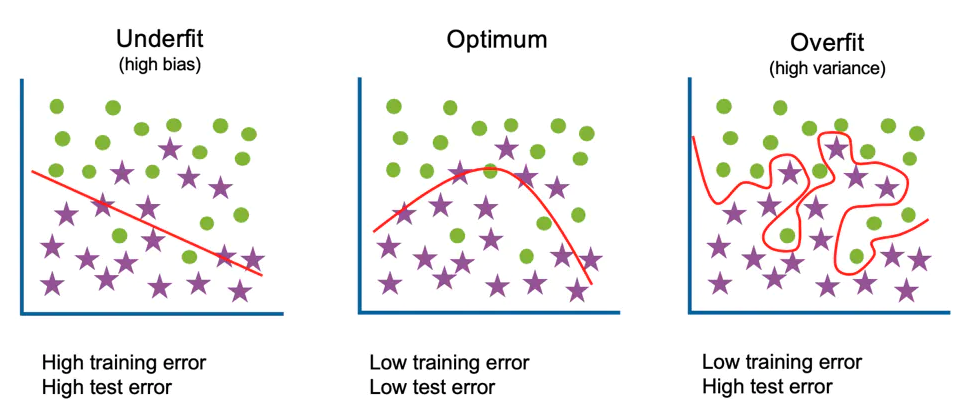
\includegraphics[width=\linewidth]{fig/overfitting.png}
    \caption{โมเดลที่มีความ Overfitting และ Underfitting กับชุดข้อมูลมากเกินไป}
    \label{fig:overfitting}
\end{figure}

\begin{description}[style=nextline]
    \item[Overfitting] โมเดลตอบสนองต่อ Noise ที่มากเกินไป ทำให้เกิดการเรียนรู้และจดจำ Noise และไม่สามารถที่จะเรียนรู้รายละเอียด%
    จริง ๆ ของข้อมูลได้ ซึ่งส่งผลให้ทำนายข้อมูลไม่ได้หรือผิดพลาดมากกว่าที่คาดไว้หรือยอมรับได้ โดยกรณีนี้โมเดลจะมีค่าความแปรปรวนของข้อมูลสูง 
    (High Variance)
    
    \item[Underfitting] โมเดลของเราไม่สามารถหาความสัมพันธ์ระหว่างอินพุต ($x$) กับเอาต์พุต ($y$) ได้เพราะว่ามีข้อมูลที่ใช้ใน%
    การเทรนน้อยเกินไปหรือดึงข้อมูลออกมาจาก Training Set ได้ไม่เพียงพอที่จะเรียนรู้ โดยในกรณีนี้โมเดลจะมีค่าความเอนเอียงสูง (High Bias)

    \item[Noisy] โมเดลไม่มี Overfitting และ Underfitting แต่ยังมีค่า Error ของการฝึกสอนที่ยังสูงอยู่มาก ซึ่งสาเหตุก็อาจจะมาจาก%
    การที่ชุดข้อมูลมี Noise มากเกินไปนั่นเอง
\end{description}

ภาพที่ \ref{fig:overfitting} แสดงการเปรียบเทียบระหว่างกรณีของ Underfitting และ Overfitting ซึ่งเป็นหนึ่งในปัญหาหลักที่มักจะพบ%
เจอได้ทั่วไปใน ML โดยเราสามารถสรุปความสัมพันธ์จากกรณีได้กล่าวได้ดังนี้

\fbox{%
\begin{minipage}{0.9\linewidth}
    \begin{align*}
        \text{Bias สูง} &\;\longleftrightarrow\; \text{Underfitting}\\
        \text{Variance สูง} &\;\longleftrightarrow\; \text{Overfitting}\\
        \text{$\sigma^2$ มาก} &\;\longleftrightarrow\; \text{Noisy Data}\\
    \end{align*}
\end{minipage}}

วิธีการจัดการกับ Overfitting แบบที่ง่ายที่สุดคือการเพิ่มจำนวนข้อมูลในการฝึกสอนโมเดล นอกจากนี้ยังมีวิธีอื่น ๆ ที่เราสามารถใช้ในการจัดการกับ%
ปัญหาข้างต้นได้เช่นเดียวกัน มีดังต่อไปนี้

%--------------------------
\subsection{Data Augmentation}
\label{ssec:data_aug}
\idxen{Data Augmentation}
%--------------------------

\begin{figure}[H]
    \centering
    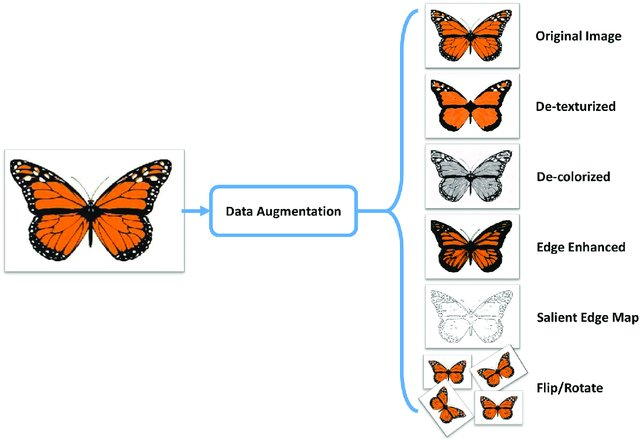
\includegraphics[width=0.9\linewidth]{fig/data_aug_butterfly.jpg}
    \caption{ตัวอย่างการทำ Data Augmentation สำหรับข้อมูลที่เป็นรูปภาพ เช่น การเปลี่ยนสี การเพิ่มความคมชัด การเพิ่ม Noise 
    (เครดิตภาพ: \textit{PLoS ONE} 12(8): e0183838)}
    \label{fig:data_aug_butterfly}
\end{figure}

วิธีการทำ Data Augmentation นั้นจะตรงข้ามกับการทำความสะอาดข้อมูล (Data Cleaning) นั่นก็คือจะเป็นวิธีที่เราจะใส่ Noise หรือสิ่งที่%
ไม่ได้เกี่ยวข้องกับข้อมูลโดยตรงเข้าไปในชุดการฝึกสอน รวมไปถึงการแก้ไขข้อมูลให้แตกต่างไปจากเดิม แต่ยังคงไว้ซึ่งลักษณะของข้อมูลนั้น 
ซึ่งการทำ Data Augmentation จะเป็นการช่วยไม่ใช่ให้เกิดการเรียนรู้ที่มันยึดติดกับชุดข้อมูลฝึกสอนมากเกินไป ในปัจจุบันวิธีการนี้ได้รับความนิยม%
เพราะสามารถทำได้ง่าย สะดวก และไม่มีความซับซ้อนในการทำ โดยมีความจำเป็นอย่างยิ่งกรณีที่ชุดข้อมูลมีขนาดเล็ก (จำนวนข้อมูลไม่เยอะ) 
แต่ต้องการนำมาใช้ในการฝึกสอนด้วยเทคนิค ML ที่ต้องการข้อมูลในปริมาณที่เยอะในการฝึกสอน เช่น Deep Learning\autocite{bengio2021}

%--------------------------
\subsection{Early Stopping}
\label{ssec:early_stop}
\idxen{Early Stopping}
%--------------------------

\begin{figure}[H]
    \centering
    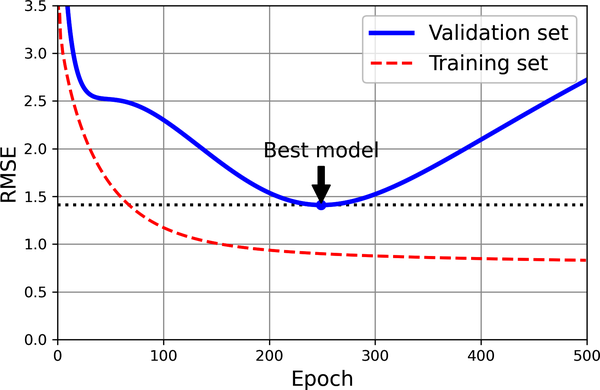
\includegraphics[width=0.9\linewidth]{fig/early_stopping.png}
    \caption{การทำ Regularization ด้วยวิธี Early Stopping สำหรับการฝึกสอนโมเดล High-degree Polynomial Regression 
    โดยใช้ Batch Gradient Descent และใช้ RMSE ในการวัดค่าความคลาดเคลื่อน (เครดิตภาพ: https://www.oreilly.com)}
    \label{fig:early_stopping}
\end{figure}

วิธี Early Stopping มีความหมายวิธีการทำงานตามชื่อเลยนั่นก็คือหยุดให้เร็วขึ้น เป็นวิธีการที่เราจะกำหนด (บังคับ) ให้การฝึกสอนหรือ Training 
นั้นหยุดก่อนที่โมเดลของเราจะเริ่มเรียนรู้ Noise ที่อยู่ภายในชุดข้อมูล แทนที่จะเรียนรู้เฉพาะชุดข้อมูลอย่างเดียว ซึ่งวิธีการนี้จะเป็นการป้องกันการเปิด 
Bias แบบตรงไปตรงมา อย่างไรก็ตามเราควรจะต้องระมัดระวังในการใช้เทคนิค Early Stopping เพราะว่าถ้าเราบังคับให้โมเดลหยุดเรียนรู้เร็วเกินไป
ปัญหาที่อาจจะเกิดขึ้นแทนการ Overfitting นั่นก็คือการ Underfitting ของโมเดล ซึ่งการเลือกจุดที่จะให้โมเดลนั้นหยุดการเรียนรู้ก็ถือว่ามีความ%
เป็น Art อย่างหนึ่ง ซึ่งจุดที่เราเลือกต้องมีความเหมาะสมระหว่าง Overfitting และ Underfitting

\noindent โค้ดของการทำ Early Stopping โดยใช้ไลบรารี่ Scikit-Learn

\begin{lstlisting}[style=MyPython]
from copy import deepcopy
from sklearn.metrics import mean_squared_error
from sklearn.preprocessing import StandardScaler

X_train, y_train, X_valid, y_valid = [...]  # split the quadratic dataset

preprocessing = make_pipeline(PolynomialFeatures(degree=90, include_bias=False),
                              StandardScaler())
X_train_prep = preprocessing.fit_transform(X_train)
X_valid_prep = preprocessing.transform(X_valid)
sgd_reg = SGDRegressor(penalty=None, eta0=0.002, random_state=42)
n_epochs = 500
best_valid_rmse = float('inf')

# Training with applying early stopping
for epoch in range(n_epochs):
    sgd_reg.partial_fit(X_train_prep, y_train)
    y_valid_predict = sgd_reg.predict(X_valid_prep)
    val_error = mean_squared_error(y_valid, y_valid_predict, squared=False)
    if val_error < best_valid_rmse:
        best_valid_rmse = val_error
        best_model = deepcopy(sgd_reg)
\end{lstlisting}

\noindent โค้ดของการสร้าง Callback ของ Early Stopping โดยใช้ไลบรารี่ TensorFlow 

\begin{lstlisting}[style=MyPython]
import tensorflow as tf

callback = tf.keras.callbacks.EarlyStopping(monitor='loss', patience=3)

model = tf.keras.models.Sequential([tf.keras.layers.Dense(10)])
model.compile(tf.keras.optimizers.SGD(), loss='mse')

history = model.fit(np.arange(100).reshape(5, 20), np.zeros(5),
                    epochs=10, batch_size=1, callbacks=[callback],
                    verbose=0)

len(history.history['loss'])  # Only 4 epochs are run.
4
\end{lstlisting}

\noindent โดย Callback จะทำการหยุดการฝึกสอน (Training) เมื่อค่า Loss ไม่มีการลดลงภายใน 3 Epochs ที่ต่อเนื่องกัน

%--------------------------
\subsection{Ensemble Method}
\label{ssec:ensemble_model}
\idxen{Ensemble Method}
%--------------------------

\begin{figure}[htbp]
    \centering
    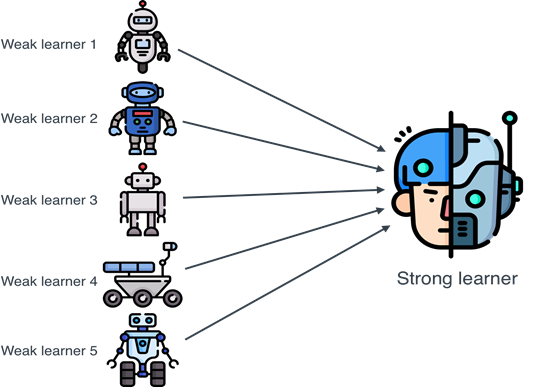
\includegraphics[width=0.9\linewidth]{fig/ensemble_method.png}
    \caption{การทำงานร่วมกันของโมเดลหลาย ๆ โมเดลโดยใช้วิธี Ensemble (เครดิตภาพ: https://www.manning.com)}
    \label{fig:ensemble_method}
\end{figure}

เทคนิคนี้เป็นการนำโมเดลหลาย ๆ โมเดลมารวมกันเพื่อที่จะทำให้ผลลัพธ์ของการทำนายคำตอบมีค่าที่ดีที่สุด โดยโมเดล ML ที่เราจะมานำผสมกันนั้น%
จะเป็นอะไรก็ได้ เช่น Linear Regression, Logistic Regression, Gaussian Process Regression ผู้อ่านสามารถดูภาพที่ 
\ref{fig:ensemble_method} ประกอบได้ โดยจะเห็นว่าเรามีโมเดลที่มีประสิทธิภาพไม่ค่อยดีนักหลาย ๆ โมเดล เราสามารถนำโมเดลเหล่านี้มา%
รวมกันเพื่อให้ได้โมเดลที่มีประสิทธิมากขึ้นได้

โดยเทคนิคย่อยของEnsemble Method ที่นิยมใช้กันนั้นมีอยู่ด้วยกัน 3 วิธี ดังนี้

\begin{itemize}[topsep=0pt]
    \item \textbf{Bagging} เราจะทำการสร้างข้อมูลประเภทเดียวกันแบบหลาย ๆ ชุด แล้วทำการทดสอบกับข้อมูลเพียงแค่บางส่วน (Subset) 
    ของชุดข้อมูล จากนั้นนำผลการทำนายของโมเดลต่าง ๆ มารวมกัน ตัวอย่างของอัลกอริทึมที่ใช้ในการเรียนรู้สำหรับเทคนิค Bagging นี้ เช่น 
    Decision Tree, Random Forest และ Extra Tree
    \idxen{Ensemble Method!Bagging}

    \item \textbf{Boosting} จะทำคล้ายกับ Bagging เลยก็คือเริ่มต้นด้วยการสร้างข้อมูลประเภทเดียวกันแบบหลาย ๆ ชุด แล้วทำการทดสอบ%
    กับข้อมูลชุดเดียวกันโดยทำการทดสอบแบบวนซ้ำ (Iteration) แล้วปรับค่าน้ำหนักเพื่อทำให้ผลการทำนายของโมเดลนั้นดีขึ้นเรื่อย ๆ ซึ่งวิธีนี้ค่อน%
    ข้างเป็นที่นิยมเพราะมีความยืดหยุ่นและใช้ได้กับทุกอัลกอริทึม นอกจากนี้ยังสามารถปรับลดค่าความคลาดเคลื่อนของ Bias ของโมเดลได้ดีอีกด้งบ 
    ตัวอย่างของอัลกอริทึมที่ใช้ในการเรียนรู้สำหรับเทคนิค Boosting นี้ เช่น AdaBoost และ Stochastic Gradient Boosting
    \idxen{Ensemble Method!Boosting}

    \item \textbf{Voting} เราจะเริ่มด้วยการสร้างโมเดลที่แตกต่างกันหลาย ๆ โมเดล เช่น Decision Tree, Support Vector Machine, 
    K-Nearest Neighbors จากนั้นทำการฝึกสอนโมเดลด้วยชุดข้อมูลชุดเดียวกันเพื่อดูผลการทำนายที่ดีที่สุดของแต่ละโมเดล แล้วใช้การโหวตผลที่%
    เหมือนกันหรือคล้ายกันเพื่อเป็นคำตอบสุดท้าย
    \idxen{Ensemble Method!Voting} 
\end{itemize}

%--------------------------
\subsection{Dropout}
\label{ssec:dropout}
\idxen{Dropout}
%--------------------------

วิธีการ Dropout เป็นเทคนิคพิเศษที่ถูกคิดค้นขึ้นมาเพื่อแก้ปัญหา Overfitting ใน Deep Learning โดยเฉพาะ ซึ่งไอเดียของเทคนิคนี้ก็คือ%
เราจะทำการตัด (Drop out หรือเอาออกไป) หน่วยการเรียนรู้ (Learning Unit หรือ Neuron) ใน Neural Network ออกไป ซึ่งจะเป็นการช่วย%
ให้โมเดลของเราลด Bias ที่เกิดจากการเรียนรู้ของข้อมูลที่มากเกินไป โดยจำนวนของ Neuron ที่จะตัดออกไปนั้นส่วนใหญ้แล้วจะคิดเป็นเปอร์เซนต์ของ
Neuron ทั้งหมด เช่น ตัดออกไป 5 เปอร์เซนต์
\idxen{Overfitting}

โค้ดของการทำ Dropout โดยใช้ไลบรารี่ TensorFlow

\begin{lstlisting}[style=MyPython]
>>> tf.random.set_seed(0)
>>> layer = tf.keras.layers.Dropout(.2, input_shape=(2,))
>>> data = np.arange(10).reshape(5, 2).astype(np.float32)
>>> print(data)
[[0. 1.]
 [2. 3.]
 [4. 5.]
 [6. 7.]
 [8. 9.]]
>>> outputs = layer(data, training=True)
>>> print(outputs)
tf.Tensor(
[[ 0.    1.25]
 [ 2.5   3.75]
 [ 5.    6.25]
 [ 7.5   8.75]
 [10.    0.  ]], shape=(5, 2), dtype=float32)
\end{lstlisting}

%--------------------------
\subsection{L1 Regularization}
\label{ssec:l1_reg}
\idxen{Regularization!L1 (LASSO)}
%--------------------------

ตามที่เราได้ศึกษาเรื่อง L1 กันไปแล้วในบทที่ \ref{ch:kernel} เราสามารถทำการปรับปรุง Loss Function ของเราได้ด้วยการเพิ่มพารามิเตอร์%
แบบพิเศษเข้าไป นั่นก็คือการใส่การลงโทษหรือ Penalty ให้กับการเรียนรู้ของโมเดล โดยการปรับพารามิเตอร์ $\lambda$ (ในบทที่ \ref{ch:kernel}
จะใช้ตัวแปร $\alpha$ ซึ่งมีความหมายเหมือนกัน) ให้เพิ่มขึ้นนั้นจะเป็นการลด Variance แต่ในขณะเดียวกันก็จะเป็นการเพิ่ม Bias โดยใน 
Linear Regression นั้นเราจะเรียก Regularization แบบ L1 ว่า LASSO

\begin{equation}
    L = \frac{1}{N}\sum_i^N \left[y_i - \hat{f}(\vec{x}_i, \vec{w}, b)\right]^2 + \lambda \sum_k \left|w_k\right|
\end{equation}

%--------------------------
\subsection{L2 Regularization}
\label{ssec:l2_reg}
\idxen{Regularization!L2 (Ridge)}
%--------------------------

สำหรับ Regularization แบบ L2 นั้นก็จะมีความคล้ายกับ L1 มาก ซึ่งวิธีนี้ในการทำ Linear Regression จะมีชื่อเรียกว่า Ridge Regression

\begin{equation}
    L = \frac{1}{N}\sum_i^N \left[y_i - \hat{f}(\vec{x}_i, \vec{w}, b)\right]^2 + \lambda \sum_k w_k^2
\end{equation}

สำหรับการเลือก Regularization นั้น ผู้เขียนขอยกประโยคของศาสตราจารย์ Frank Harrell ที่ได้แนะนำการเลือก L1 และ L2 ไว้ดังนี้%
\footnote{อ้างอิง \url{https://stats.stackexchange.com/a/184022/283188}}

\begin{framed}
    \enquote{Generally speaking if you want optimum prediction use L2. 
    If you want parsimony at some sacrifice of predictive discrimination use L1. 
    But note that the parsimony can be illusory, e.g., repeating the \textit{lasso} 
    process using the bootstrap will often reveal significant instability 
    in the list of features \enquote{selected} especially when predictors are 
    correlated with each other.}
\end{framed}

ซึ่งตีความได้คร่าว ๆ ว่าถ้าหากต้องการการทำนายที่เหมาะสมที่สุดให้ใช้ L2 หรือ Ridge Regression แต่ถ้าหากต้องการทำให้การจำแนกเชิงพยากรณ์
(Predictive Discrimination) มีความสม่ำเสมอกันสำหรับทุก ๆ Feature ให้ใช้ L1 หรือ Lasso Regression แต่ควรเข้าใจไว้ด้วยว่าการ%
ใช้ L1 สามารถทำให้เกิดปัญหาได้ เช่น การทำ Lasso Regression โดยใช้เทคนิค Bootstrap (การ Sample ตัวอย่างจากชุดข้อมูล)
